\chapter{Implementación}

A continuación se detallan la instalación, configuración así como el desarrollo de los elementos que componenen el sistema. A modo de resumen los puntos serán los siguientes:

\begin{itemize}
	\item Descripción de las tecnologías seleccionadas.
	\item Instalación y configuración de Raspberry Pi.
	\item Instalación y configuración de KAA.
	\item Instalación y configuración de Apache Cassandra.
	\item Desarrollo del módulo de detección de vehículos.
	\item Desarrollo de la plataforma web.
	\item Instalación y configuración de Apache Zeppelin.
\end{itemize}

\newpage

\section{ Descripción de las tecnologías seleccionadas}

Éste apartado detalla las tecnologías seleccionadas así como las que finalmente fueron descartadas.

A lo largo del desarrollo del proyecto el diseño ha ido cambiando progresivamente debido a que el número de elementos que lo componen deben cohesionarse para trabajar sobre la solución, siendo éste uno de los mayores problemas encontrados ya que al elegir una tecnología se deben desarrollar una serie de pruebas para confirmar que es la óptima de cara al diseño final.

\newpage

\subsection{Plataforma IOT}

Éste aspecto ha sio uno de los más relevantes, el cual ha marcado el funcionamiento final de la aplicación. Existen muchas alternativas debido al auge de IOT no obstante la plataforma debía cumplir una serie de premisas enumeradas a continuación:

\begin{itemize}
    \item \textbf{Open Source: } para mantener el licenciamiento de la aplicación final.
    \item \textbf{Independiente: } esto es, debe ser un sistema instalable en un servidor propio sin necesidad de depender de servidores de terceros.
    \item \textbf{Soporte para Raspberry Pi: } es obvio que debe poderse integrar con nuestro dispositivo receptor.
    \item \textbf{Número de dispositivos ilimitado: } esto nos permitirá cumplir con el requisito de que cualquiera pueda proveer datos a la aplicación.
    \item \textbf{Documentación: } es un elemento importante, más aún, cuando se desconoce la materia.
\end{itemize}

El abanico de posibilidades es muy extenso pero no todas cumplen con los requisitos deseados, las opciones finalmente descartadas fueron:
\begin{itemize}
    \item \textbf{Thinger.io} cubre alguna de las necesidades que se precisan sin embargo la documentación muy es pobre.
    \item \textbf{IBM Watson} es un candidato a tener en cuenta sin embargo trabajar en servidores de terceros y ser de pago ha sido un factor decisivo para descartarlo.
    \item \textbf{AWS IOT} de similares características a IBM Watson, ha sido descartado por las mismas razones que el anterior.
    \item \textbf{Node-RED} es el perfil que más se acerca a lo requierido, no ha sido elegido porque la alternativa finalmente escogida tiene una comunidad más activa y por tanto la documentación es mejor.
\end{itemize}

\bigskip

\newpage

Esto nos lleva a \textbf{KAA} (\url{http://www.kaaproject.org/}) la cual cumple todos los requisitos deseados completamente.

\begin{figure}[ht]
  \begin{center}
    
\includegraphics[scale=0.10]{../images/kaa/logo.png}
    \label{fig:kaalog}
	\end{center}
\end{figure}

\begin{quote}\textit{''Kaa is a feature-rich, open-source IoT middleware platform for rapid development of the Internet of Things solutions, IoT applications, and smart products.''}
\newline
\url{http://www.kaaproject.org/}
\end{quote}

KAA provee una imagen para ser instalada sobre Amazon EC2 lo que simplifica mucho la tarea de instalación y configuración, además cuenta con una extensa documentación, webinars y ejemplos que han sido de gran ayuda a la hora del desarrollo.

Su arquitectura se puede ver en la \textit{figura 6.1}, actúa como middleware entre nuestra aplicación y los dispositivos que se desean conectar, para ello cuenta con un servidor web (instalado en la imagen que proveen) en el cual podemos configurar las aplicaciones que deseemos. Para cada una de éstas aplicaciones se genera un SDK en el lenguaje deseado el cual será usado para enviar ó recibir información.

\begin{figure}[ht]
  \begin{center}
    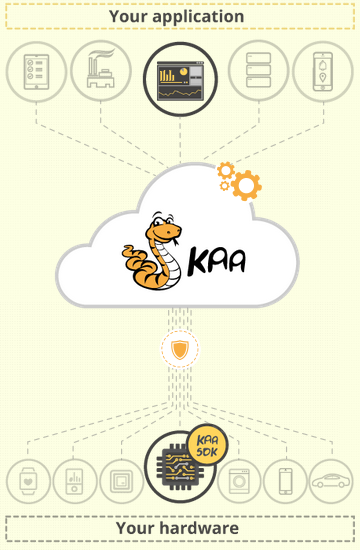
\includegraphics[scale=0.40]{../images/kaa/arqui.png}
		\caption{Arquitectura de KAA}
    \label{fig:kaalog}
	\end{center}
\end{figure}


\newpage

\subsection{Dispositivo receptor}

En éste aspecto no había muchas dudas en cuanto a las tecnologías a usar. Por una parte tenemos Raspbian, el sistema operativo oficial de Raspberry Pi basado en Debian. Usar algún otro sistema operativo ARM implicaría la incertidumbre sobre cualquier tipo de error en gran parte por el aspecto de los drivers.

\bigskip
Por otra parte tenemos el software desarrollado que se ejecuta en el dispositivo. Al igual que con el sistema operativo, el lenguaje de programación elegido desde un principio fue \textbf{Python} por su sencillez y número de bibliotecas. A medida que el desarrollo ha ido evolucionando Python ha demostrado ser el mejor candidato para el uso que se le pretendía dar, en gran parte gracias a la biblioteca \textbf{SoundDevice} que nos proporciona una manera realmente fácil de acceder y capturar datos de las interfaces de audio además de contar con numerosos ejemplos los cuales han sido de gran ayuda.

\bigskip
Por último, el dispositivo necesita hacer uso del SDK generado por KAA. Existen varias alternativas a la hora de generarlo y la más atractiva resultó ser \textbf{Java}. La interacción entre Python y Java se detallará más adelante.

\subsection{Almacenamiento de información}

Para almacenar datos de manera masiva existen varias alternativas como son Apache HBase, MongoDB, Apache Cassandra, Hive ó Redis. En éste aspecto la diferencia entre unas y otras es menores sin embargo hay una de ellas que destaca respecto a las otras por la facilidad de integración con KAA, es \textbf{Apache Cassandra} (\url{http://cassandra.apache.org/}).

\begin{figure}[!ht]
  \begin{center}
    
\includegraphics[scale=0.60]{../images/cassandra/logo.jpg}
    \label{fig:cassalog}
	\end{center}
\end{figure}

\begin{quote}\textit{ ''... is the right choice when you need scalability and high availability without compromising performance... Is best-in-class, providing lower latency for your users...''
}
\newline
\url{http://cassandra.apache.org/}
\end{quote}

Tras una breve documentación acerca de Cassandra se vió que era un software con unas características y una potencia a tener muy en cuenta además de su facilidad integración con KAA como se ha mencionado anteriormente, también se pueden definir funciones personalizadas en el lenguaje deseado y tiene una línea de comandos amigable. El lenguaje de consultas es CQL y su sintaxis no difiere mucho del resto de SGBD.


\subsection{Representación de información}

En éste apartado las opciones a tener en cuenta era Apache-Zeppelin y Jupyter. Ambas herramientas tienen el papel de representar la información que va a almacenar Cassandra. La integración entre la base de datos y Zeppelin se hace de una manera sencilla (ambas pertenecen a Apache) así como las consultas y visualización de datos, es por eso por lo que finalmente se optó por la opción de \textbf{Apache Zeppelin} (\url{https://zeppelin.apache.org/}).

\begin{figure}[!ht]
  \begin{center}
    
\includegraphics[scale=0.60]{../images/zeppelin/logo.png}
    \label{fig:zepplog}
	\end{center}
\end{figure}

\begin{quote}\textit{ ''A web-based notebook that enables interactive data analytics.
You can make beautiful data-driven, interactive and collaborative documents...''
}
\newline
\url{https://zeppelin.apache.org/}
\end{quote}

Apache Zeppelin nos va a permitir configurar una serie de Notebooks en forma de plataforma web en los que podremos realizar consultas a Cassandra para obtener los datos almacenados de los dispositivos receptores. Los datos se obtendrán mediante consultas CQL y podrán ser representados de varias formas, incluyendo distintos tipos de gráficos así como permitiendo la exportación de los mismos.

\newpage

\subsection{Plataforma Web de RSMap}

Para la plataforma web aunque las opciones eran varias en términos de lenguajes y frameworks. Finalmente la tecnología usada será Django que es un framework para aplicaciones web en Python.

\begin{figure}[!ht]
  \begin{center}
    
\includegraphics[scale=0.1]{../images/web/django-logo.png}
    \label{fig:drflog}
	\end{center}
\end{figure}

Las principales causas para la elección son la familiaridad con el mismo, que trabaja bajo el modelo Vista-Controlador, su documentación y el módulo Django-Rest-Framework que permite a los dispositivos comunicarse directamente con la web que será la encargada de representar en un mapa pequeños iconos que indiquen el paso de un vehículo.

El mapa es provisto por Google Maps.  Para ofrecer una navegación fluida concretamente en la sección del mapa se hará uso de jQuery y AJAX que nos sirven métodos para actualizar la información en el mismo mapa de manera automática y sin necesidad de recargar la página para ver los cambios.

El aspecto visual queda resuelto gracias a la librería Bootstrap (css) y una plantilla (html5) predefinida Open Source sobre la que efectuaremos las modificaciones necesarias para adaptarla a las necesidades de RSMap.

\section{Instalación y configuración de Raspberry Pi}

\subsection{Instalación}

En primer lugar se indica como instalar Raspbian en nuestra Raspberry Pi Jessie (basado en Debian), ésta ha sido la opción seleccionada como SO debido a que es el sistema oficial que provee Raspberry Pi.

\bigskip

El primer paso es descargarse la imagen de los servidores oficiales, la imagen usada se puede encontrar en \url{https://downloads.raspberrypi.org/raspbian/images/raspbian-2016-05-31/}

\begin{lstlisting}[language=bash,caption={Copia de Raspbian en tarjeta s y usb},label={lst:pi1}]
# muestra los discos del sistema
$ lsblk
# copia la imagen en el dispositivo /dev/sdb (tarjeta sd)
$ sudo dd bs=1M if=2016-05-27-raspbian-jessie.img of=/dev/sdb
# copia la particion del sistema en /dev/sdc (usb)
$ sudo dd bs=1M if=/dev/sdb2 of=/dev/sdc
\end{lstlisting}

\bigskip

Ahora editamos el archivo \textbf{/dev/sdb/boot/cmdline.txt} y añadimos la siguiente línea para que el sistema sólo use la tarjeta SD para arrancar y el dispositivo usb como disco del sistema, ésto aumentará la velocidad de lectura considerablemente:


\begin{lstlisting}[language=bash,caption={Modificando el dispositivo de arranque de Raspbian},label={lst:pi2}]
smsc95xx.turbo_mode=N dwc_otg.lpm_enable=0 console=ttyAMA0,115200 kgdboc=ttyAMA0,115200 console=tty1 root=/dev/sda1 rootfstype=ext4 elevator=noop rootwait # /dev/sda1 point to our USB drive
\end{lstlisting}

\bigskip

\subsection{Configuración}

Vamos a instalar el software necesario para interactuar con la tarjeta de sonio además de comprobar si el sistema la soporta y en caso afirmativo, establecerla como dispositivo de audio por defecto lo cual nos permitirá trabajar con ella después de cada reinicio ó apagado del dispositivo.

\begin{lstlisting}[language=bash,caption={Instalación del paquete alsa-utils},label={lst:pi3}]
$ sudo apt-get install alsa-utils
\end{lstlisting}

\begin{lstlisting}[language=bash,caption={Comprobano que el dispositivo es reconocido},label={lst:pi3}]
$ lsusb
Bus 001 Device 005: ID 0d8c:000c C-Media Electronics, Inc. Audio Adapter
Bus 001 Device 004: ID 0781:5567 SanDisk Corp. Cruzer Blade
Bus 001 Device 003: ID 0424:ec00 Standard Microsystems Corp. SMSC9512/9514 Fast Ethernet Adapter
Bus 001 Device 002: ID 0424:9514 Standard Microsystems Corp.
Bus 001 Device 001: ID 1d6b:0002 Linux Foundation 2.0 root hub
\end{lstlisting}

\begin{lstlisting}[language=bash,caption={Identificando los dispositivos de sonido disponibles en el sistema},label={lst:pi4}]
$ aplay -l
**** List of PLAYBACK Hardware Devices ****
card 0: ALSA [bcm2835 ALSA], device 0: bcm2835 ALSA [bcm2835 ALSA]
  Subdevices: 8/8
  Subdevice #0: subdevice #0
  Subdevice #1: subdevice #1
  Subdevice #2: subdevice #2
  Subdevice #3: subdevice #3
  Subdevice #4: subdevice #4
  Subdevice #5: subdevice #5
  Subdevice #6: subdevice #6
  Subdevice #7: subdevice #7
card 0: ALSA [bcm2835 ALSA], device 1: bcm2835 ALSA [bcm2835 IEC958/HDMI]
  Subdevices: 1/1
  Subdevice #0: subdevice #0
card 1: Set [C-Media USB Headphone Set], device 0: USB Audio [USB Audio]
  Subdevices: 1/1
  Subdevice #0: subdevice #0
	\end{lstlisting}

\bigskip

En éste caso el dispositivo se llama \textit{C-Media USB Headphone SetC-Media USB Headphone Set} cuyo identificador es 1, para establecerla como dispositivo de audio por defecto editamos \textit{/home/user/.asoundrc} con el siguiente contenido:


\begin{lstlisting}[language=bash,caption={Comprobano que el dispositivo es reconocido},label={lst:pi5}]
    pcm.!default {
      type hw
      card 1
  }

  ctl.!default {
      type hw
      card 1
  }
\end{lstlisting}

\section{Instalación y configuración de KAA}

\subsection{Instalación}

Para la instalación de KAA nos bastará con Amazon EC2, ya que el sistema de imágenes de SO contiene la versión más actual de KAA, los pasos a seguir son los siguientes:

Necesitamos una cuenta en Amazon EC2, tras registrarnos nos dirigimos al panel principal, y en el apartado \textit{INSTANCES} seleccionamos, \textit{Launch Instance} para crear una nueva máquina.

\begin{figure}[!ht]
  \begin{center}
    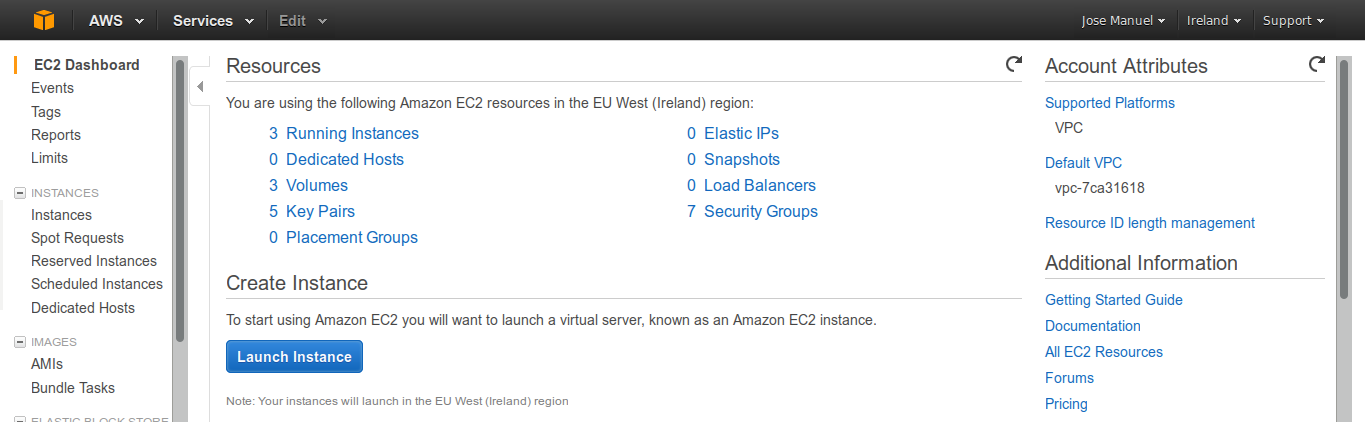
\includegraphics[scale=0.30]{../images/kaa/1.png}
		\caption{Dashboard de AmazonEC2}
    \label{fig:1}
	\end{center}
\end{figure}

\newpage

El segundo paso es dirigirse a \textit{Community AMIs} y en el cuadro de búsqueda escribimos \textit{kaa-sandbox}. Lo recomendable es usar la última versión, en éste caso se ha tomado la \textbf{versión 0.9}.

\begin{figure}[!ht]
  \begin{center}
    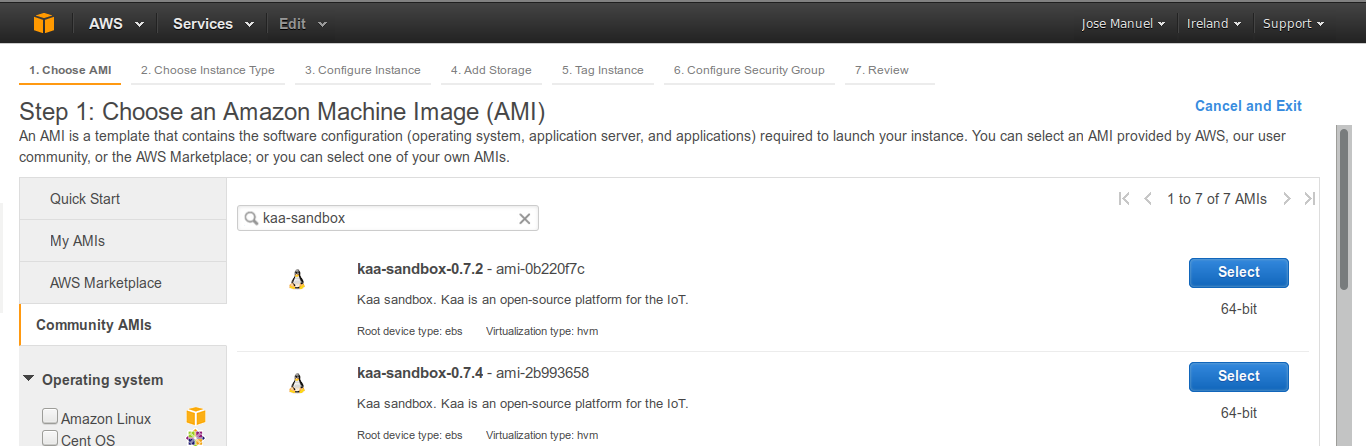
\includegraphics[scale=0.30]{../images/kaa/2.png}
		\caption{}
    \label{Instancias preconfiguradas de Kaa en EC2}
	\end{center}
\end{figure}

\newpage

Ahora debemos elegir el tipo de instancia, esto va directamente relacionado con la potencia de la misma. En un principio nos puede valer con las instancias de tipo \textit{free tier} y configurar la escalabilidad a medida de nuestras necesidades.

\begin{figure}[!ht]
  \begin{center}
    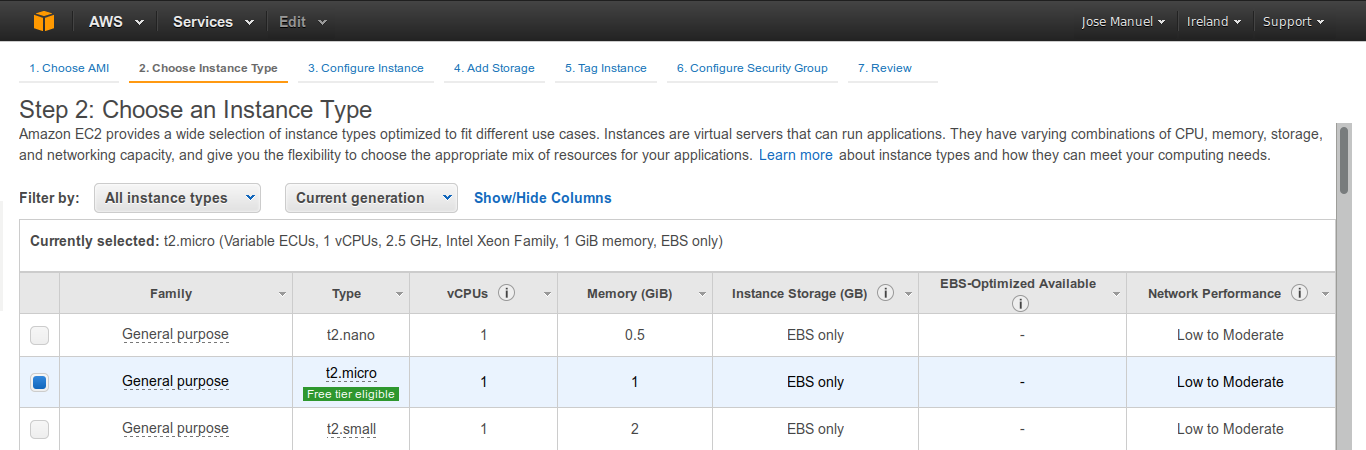
\includegraphics[scale=0.30]{../images/kaa/3.png}
		\caption{Selección del tipo de instancia}
    \label{fig:kaa}
	\end{center}
\end{figure}

En el siguiente paso podemos configurar algunas opciones relativas a la máquina, las que están por defecto son adecuadas por tanto no es necesario cambiar ninguna de ellas.

\begin{figure}[!ht]
  \begin{center}
    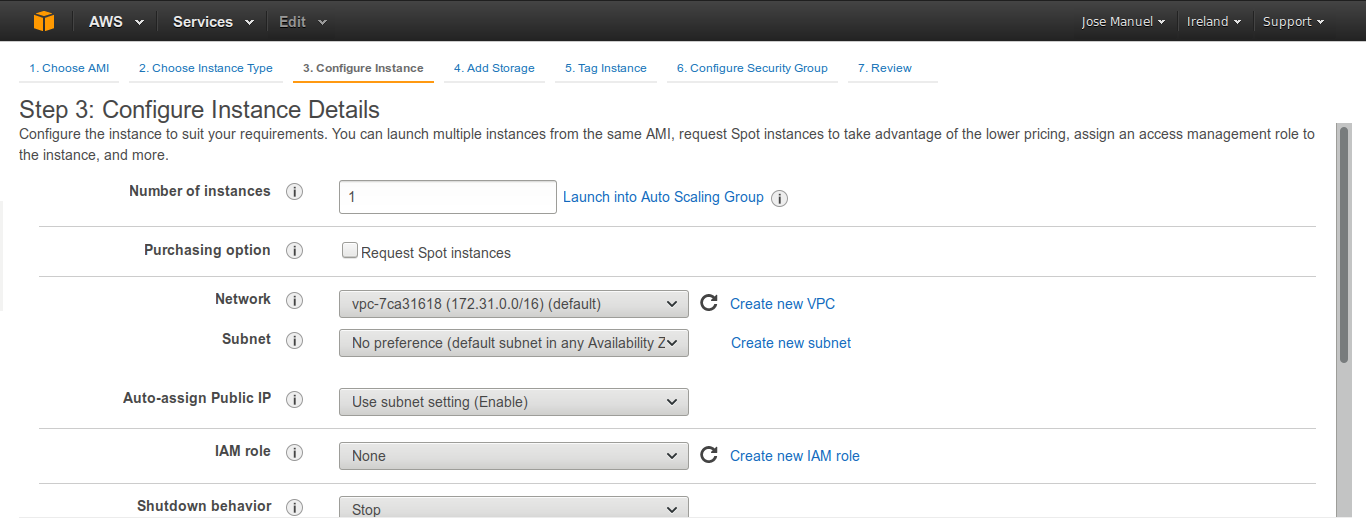
\includegraphics[scale=0.30]{../images/kaa/4.png}
		\caption{Configurar detalles de la instancia}
    \label{fig:kaa}
	\end{center}
\end{figure}

\newpage

El siguiente diálogo nos da la opción de configurar el almacenamiento, debido a que trabajamos en una instancia de tipo \textit{free tier} estamos restringidos a un tipo determinado de almacenamiento que al igual que el tipo de instancia, es suficiente por el momento.

\begin{figure}[!ht]
  \begin{center}
    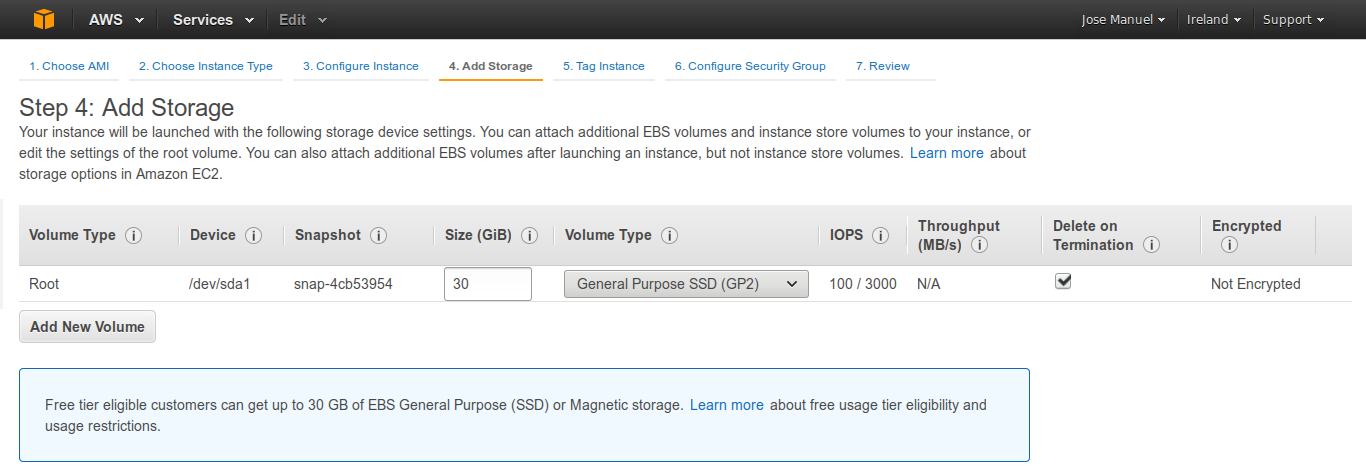
\includegraphics[scale=0.30]{../images/kaa/5.png}
		\caption{Selección de almacenamiento}
    \label{fig:kaa}
	\end{center}
\end{figure}

Los \textit{Security group} hacen referencia a la configuración de puertos, en la documentación de KAA se especifica cual debe ser, para el correcto funcionamiento y tiene una estructura como la de la \textit{ figura 6.7}.

\begin{figure}[!ht]
  \begin{center}
    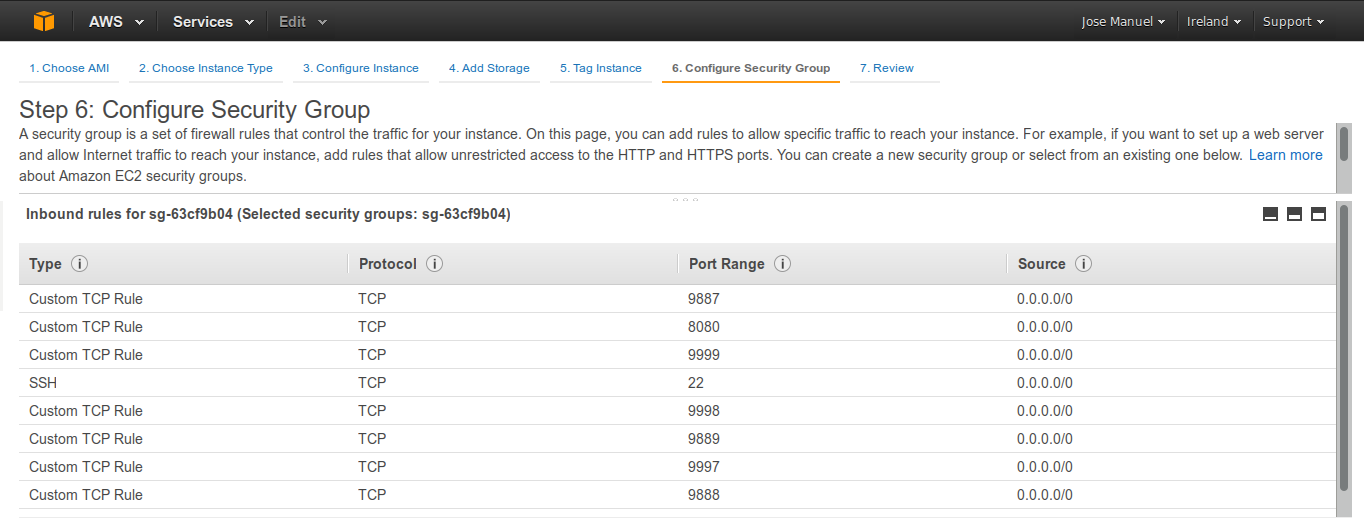
\includegraphics[scale=0.30]{../images/kaa/6.png}
		\caption{Configuración de puertos}
    \label{fig:kaa}
	\end{center}
\end{figure}

\newpage

Por último y no menos importante, debemos crear un par de llaves ó asignar uno existente. Ésto nos va a permitir conectarnos através de \textit{SSH} a la máquina en cualquier momento, si perdemos este par de claves perderemos el acceso a la máquina.

\begin{figure}[!ht]
  \begin{center}
    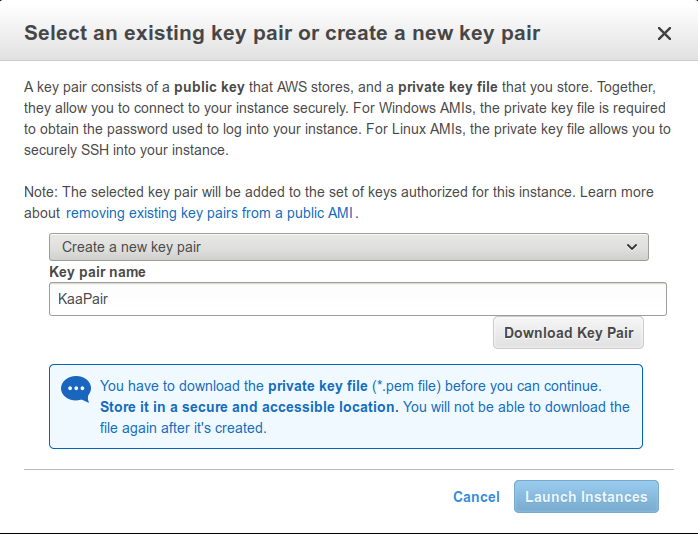
\includegraphics[scale=0.45]{../images/kaa/7.png}
		\caption{Creación de claves}
    \label{fig:kaa}
	\end{center}
\end{figure}

\subsection{Configuración}

Una vez tenemos el servicio instalado la configuración es trivial debido a que KAA provee un servicio web através del que definimos todo lo necesario.

Antes de empezar merece la pena destacar que existe 3 tipos de usuarios en KAA:

\begin{itemize}
	\item \textbf{Admin: } puede dar de alta Tenant admins.
	\item \textbf{Tenant admin: } puede dar de alta aplicaciones y Tenant developers.
	\item \textbf{Tenant developer:} puede configurar las aplicaciones y generar SDK's.
\end{itemize}

\bigskip

El primer paso es establecer la ip pública de KAA, accediendo desde el menú \textit{management}.

\begin{figure}[!ht]
  \begin{center}
    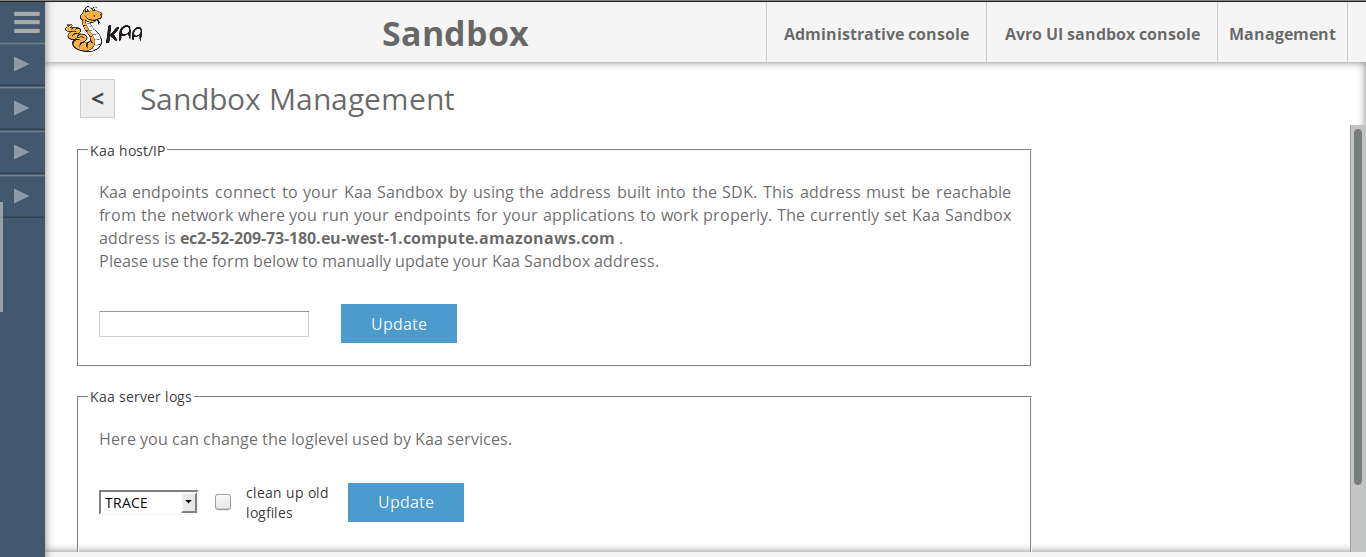
\includegraphics[scale=0.30]{../images/kaa/8.png}
		\caption{Sección Management}
    \label{fig:kaa}
	\end{center}
\end{figure}

\newpage

Ahora nos dirigimos a \textit{Administrative console} y nos logeamos como Tenant admin para dar de alta una nueva aplicación.

El tipo de credencial seleccionado será \textit{Trusful} de esta forma permitiremos a cualquier cliente conectarse a nuestra aplicación sin necesidad de autentificarse.

\begin{figure}[!ht]
  \begin{center}
    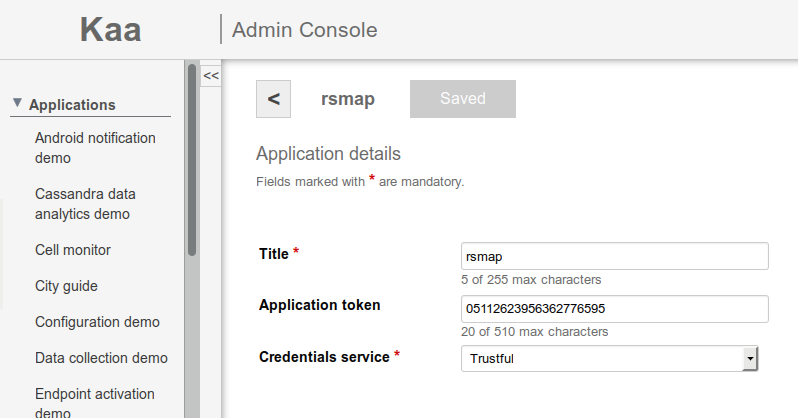
\includegraphics[scale=0.50]{../images/kaa/11.png}
		\caption{Creación de la nueva aplicación}
    \label{fig:kaa}
	\end{center}
\end{figure}

Nos logeamos con una cuenta Tenant Developer, vamos a proceder a crear la estructura de datos que define los campos y el tipo de los mismos que pertenecerán a nuestra aplicación.

Éste paso puede hacerse desde la interfaz web o subiendo un archivo \textit{json}. En nuestro caso vamos a valernos del \textit{json} por comodidad.

\begin{figure}[!ht]
  \begin{center}
    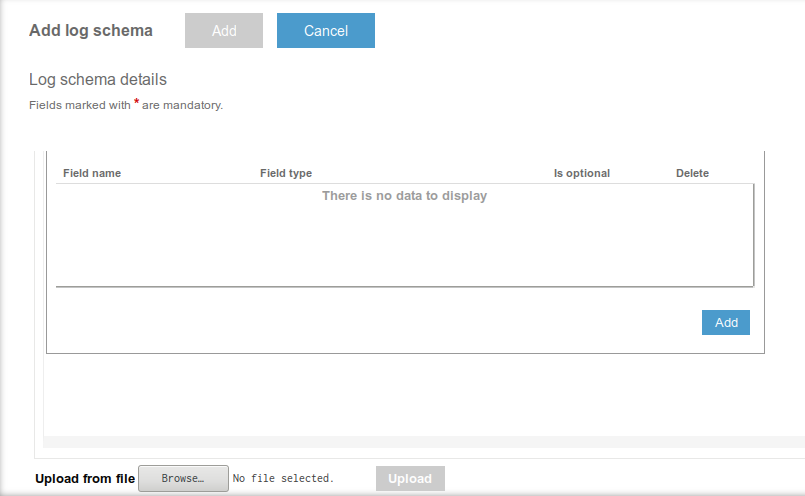
\includegraphics[scale=0.45]{../images/kaa/11-2.png}
		\caption{Definiendo esquemas de datos}
    \label{fig:kaa}
	\end{center}
\end{figure}

\newpage

Aquí se definen los campos que KAA va a proveer en el SDK generado, lo que se traduce en que éste mismo SDK nos ofrecerá una clase con los campos definidos en éste apartado. El campo \textit{namespace} indica en que paquete se encontrará la clase correspondiente al esquema definido dentro del SDK generado. KAA hace uso de Apache Avro para definir esquemas de serialización de datos. Ésto le permite manejar internamente la información almacenada en los esquemas.

\bigskip

\begin{lstlisting}[language=json,caption={Esquema de datos en JSON},label={lst:json_personal}]
{
	"type" : "record",
	"name" : "AudioReport",
	"namespace" : "org.kaaproject.kaa.schema.rsmap",
	"fields" : [ {
		"name" : "timestamp",
		"type" : "long"
	}, {
		"name" : "zoneId",
		"type" : {
			"type" : "string",
			"avro.java.string" : "String"
		}
	}, {
		"name" : "deviceId",
		"type" : {
			"type" : "string",
			"avro.java.string" : "String"
		}
	}, {
		"name" : "level",
		"type" : "double"
	} ]
}
\end{lstlisting}

Ahora ya tenemos el esquema definido en KAA como muestran la \textit{figura 6.12} y la \textit{figura 6.13}:

\begin{figure}[!ht]
  \begin{center}
    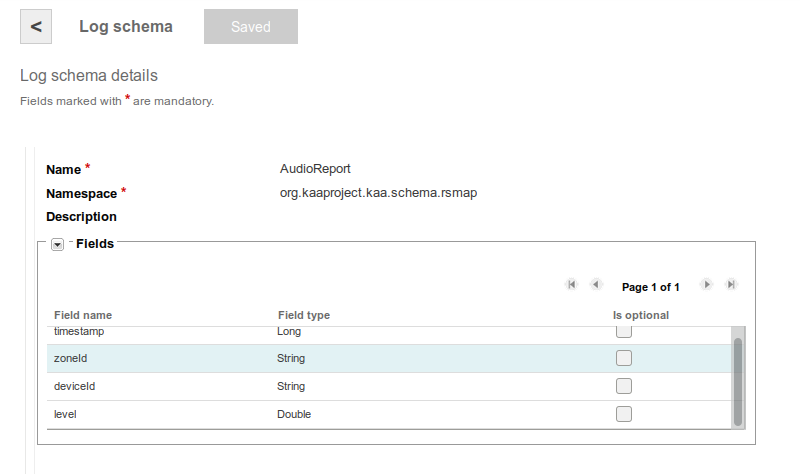
\includegraphics[scale=0.45]{../images/kaa/13.png}
		\caption{Esquema de datos definido 1}
    \label{fig:kaa}
	\end{center}
\end{figure}

\begin{figure}[!ht]
  \begin{center}
    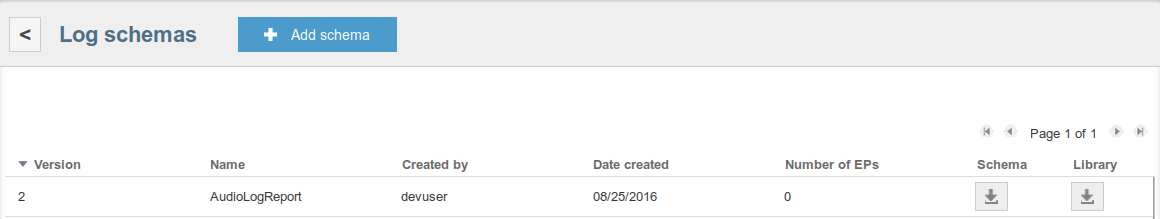
\includegraphics[scale=0.30]{../images/kaa/14.png}
		\caption{Esquema de datos definido 2}
    \label{fig:kaa}
	\end{center}
\end{figure}

\newpage

\newpage
\newpage
\newpage

\section{Instalación y configuración de Apache Cassandra.}

\subsection{Instalación}

El proceso para definir la máquina virtual que contiene Cassandra es el mismo que el de KAA a excepción de dos puntos, el primero es el tipo de instancia. Dentro de \textit{Community AMIs} debemos buscar \texit{Cassandra} y elegir la versión más reciente.

\begin{figure}[!ht]
  \begin{center}
    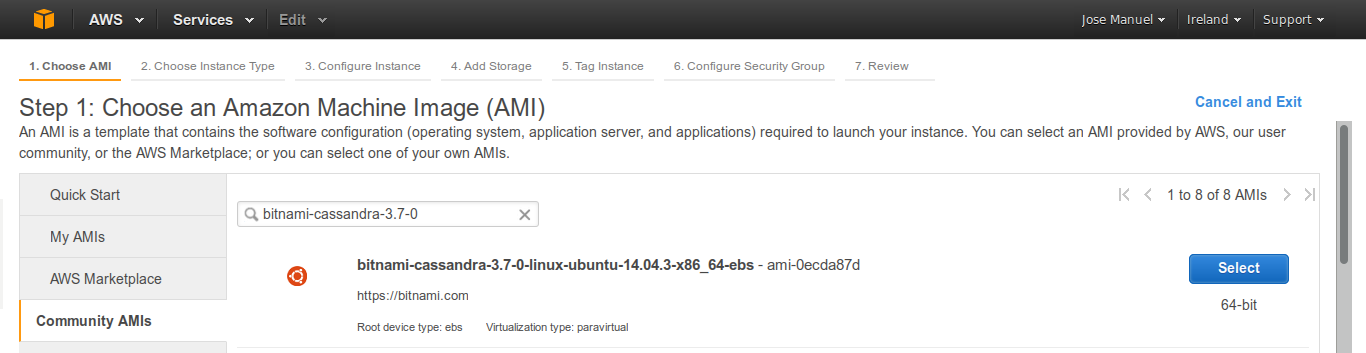
\includegraphics[scale=0.30]{../images/cassandra/1.png}
		\caption{Imagen de Cassandra en EC2}
    \label{fig:kaa}
	\end{center}
\end{figure}

El otro punto que difiere es el \textit{Security Group}, dado que los puertos que necesitamos son distintos la configuración debe quedar tal que así:

\begin{figure}[!ht]
  \begin{center}
    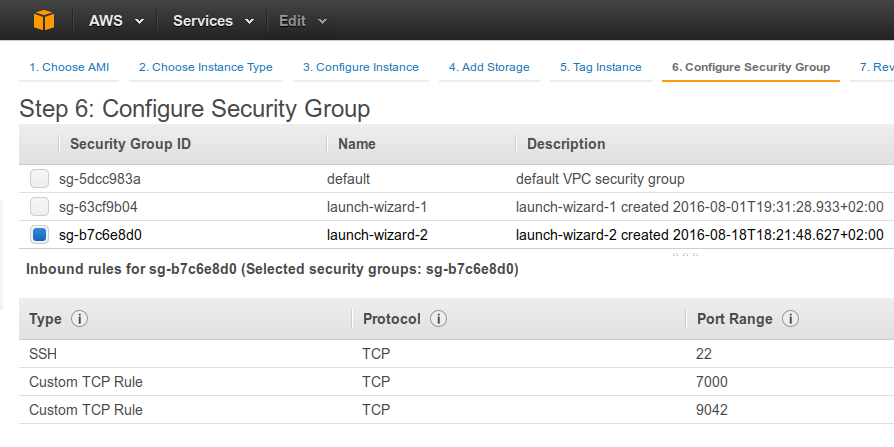
\includegraphics[scale=0.30]{../images/cassandra/2.png}
		\caption{Security Group para Cassandra}
    \label{fig:kaa}
	\end{center}
\end{figure}

\newpage

\subsection{Configuración}

Para comprobar que funciona correctamente accedemos mediante \textit{SSH} y nos logeamos en la shell de Cassandra haciendo uso del comando \textbf{cqlsh} como indica la \textit{figura 6.16}.

\begin{figure}[!ht]
  \begin{center}
    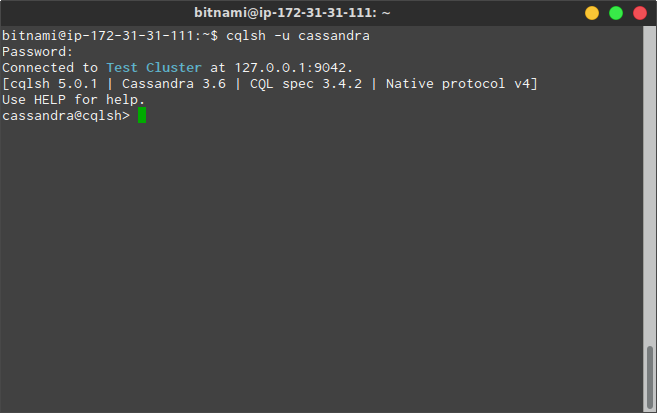
\includegraphics[scale=0.55]{../images/cassandra/3.png}
		\caption{Accediendo al servidor de Cassandra}
    \label{fig:kaa}
	\end{center}
\end{figure}

\newpage

Vamos a crear un \textit{Keyspace} que contendrá las tablas de nuestra aplicación, para ello usamos la siguiente sentencia:

\begin{lstlisting}[language=json,caption={Keyspace en Cassandra},label={lst:json_personal}]

CREATE KEYSPACE rsmapv0 WITH replication = {
	'class': 'SimpleStrategy',
	'replication_factor': 1
};

\end{lstlisting}

\textit{SingleStrategy} indica que sólo usaremos un \textit{Datacenter} y en \textit{replication factor} se indica el número de nodos de copia que queremos establecer.

\newpage

Ahora es momento de volver a KAA y definir el \textit{LogAppender} que se encargará de decirle a los clientes cómo y donde tienen que enviar los datos mediante el SDK. En nuestro caso será la base de datos que acabamos de configurar. Ésto lo haremos en la sección de Log appenders mediante un fichero \textit{json} con la siguiente estructura:


\begin{lstlisting}[language=json,caption={Esquema de log appender en JSON},label={lst:json_personal}]

{
   "cassandraServers":[
      {
         "host":"ec2-52-210-20-84.eu-west-1.compute.amazonaws.com",
         "port":9042
      }
   ],
   "cassandraCredential":{
      "org.kaaproject.kaa.server.appenders.cassandra.config.gen.CassandraCredential":{
         "user":"####",
         "password":"####"
      }
   },
   "keySpace":"rsmapv0",
   "tableNamePattern":"rows",
   "columnMapping":[
      {
         "type":"EVENT_FIELD",
         "value":{
            "string":"zoneId"
         },
         "columnName":"zone_Id",
         "columnType":"TEXT",
         "partitionKey":true,
         "clusteringKey":false
      },
      {
         "type":"EVENT_FIELD",
         "value":{
            "string":"timestamp"
         },
         "columnName":"timestamp",
         "columnType":"BIGINT",
         "partitionKey":false,
         "clusteringKey":true
      },
      {
         "type":"EVENT_FIELD",
         "value":{
            "string":"deviceId"
         },
         "columnName":"device_Id",
         "columnType":"TEXT",
         "partitionKey":false,
         "clusteringKey":true
      },
      {
         "type":"EVENT_FIELD",
         "value":{
            "string":"level"
         },
         "columnName":"level",
         "columnType":"DOUBLE",
         "partitionKey":false,
         "clusteringKey":false
      }
   ],
   "clusteringMapping":[
      {
         "columnName":"timestamp",
         "order":"DESC"
      }
   ],
   "cassandraBatchType":{
      "org.kaaproject.kaa.server.appenders.cassandra.config.gen.CassandraBatchType":"UNLOGGED"
   },
   "cassandraSocketOption":null,
   "executorThreadPoolSize":1,
   "callbackThreadPoolSize":2,
   "dataTTL":0,
   "cassandraWriteConsistencyLevel":{
      "org.kaaproject.kaa.server.appenders.cassandra.config.gen.CassandraWriteConsistencyLevel":"ONE"
   },
   "cassandraCompression":{
      "org.kaaproject.kaa.server.appenders.cassandra.config.gen.CassandraCompression":"NONE"
   },
   "cassandraExecuteRequestType":{
      "org.kaaproject.kaa.server.appenders.cassandra.config.gen.CassandraExecuteRequestType":"SYNC"
   },
   "minLogSchemaVersion":1,
   "maxLogSchemaVersion":2147483647,
   "pluginTypeName":"Cassandra",
   "pluginClassName":"org.kaaproject.kaa.server.appenders.cassandra.appender.CassandraLogAppender",
   "headerStructure":[

   ]
}

\end{lstlisting}

Los campos a tener en consideración en este archivo son los siguientes:

\begin{itemize}
	\item \textbf{Host:} hace referencia a la IP de Cassandra.
	\item \textbf{Port:} puerto de Cassandra.
	\item \textbf{User:} usuario de Cassandra.
	\item \textbf{Password:} contraseña de Cassandra.
	\item \textbf{keySpace:} keySpace de Cassandra.
	\item \textbf{tableNamePattern:} nombre de la tabla a crear.
	\item \textbf{columnMapping:} equivalencia entre los campos definidos en el esquema y las columnas que contendrá cada entrada en la base de datos.
\end{itemize}


Por tanto en éste fichero se especifica el usuario y la contraseña de Cassandra que han sido ocultados por seguridad, la IP pública del servidor Cassandra y campos del final indican la equivalencia entre los campos de esquema creado anteriormente y las tablas en Cassandra.

Una vez generemos el esquema, KAA se conectará a Cassandra y creará las tablas según el formato que le hemos indicado en el mapa \textit{columnMapping}.

\bigskip

Un factor importante es el diseño de las tablas, pues las consultas en Cassandra son dependientes de la estructura de la base de datos. El tipo de campos que determinan la estructura de la tabla son los siguientes:

\begin{itemize}
\item \textbf{partitionKey, } que es la responsable de la distribución de los datos entre los nodos de Cassandra.
\item \textbf{clusteringKey, } que se usa para ordenar los elementos dentro de una partición.
\end{itemize}

En el caso de RSMap se usa el campo \textit{zoneId} como \textit{partition key} y \textit{timestamp y deviceId} como \textit{clustering key} lo que nos garantiza que podremos hacer consultas del tipo:


\begin{lstlisting}[language=cql,caption={Mécanica de consultas en CQL según la estructura de tablas},label={lst:json_personal}]

SELECT * FROM abc WHERE partitionKey = 'X';
SELECT * FROM table WHERE partitionKey = 'X' AND clusteringKey  = 'Y';

\end{lstlisting}

\bigskip

Tras guardar el \textit{log appender} podemos comprobar como se ha creao la tabla \textit{rows} dentro del keyspace \textit{rsmapv0}. Para realizar ésta comprobación accedemos a la shell de Cassandra como muestra la \textit{figura 6.17	}.

\begin{figure}[!ht]
  \begin{center}
    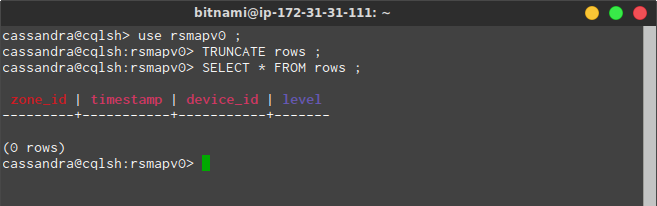
\includegraphics[scale=0.65]{../images/cassandra/4.png}
		\caption{Comprobación de las tablas creadas}
    \label{fig:kaa}
	\end{center}
\end{figure}

\newpage

Cuando la tabla contiene datos la consulta se muestra así:

\begin{figure}[!ht]
  \begin{center}
    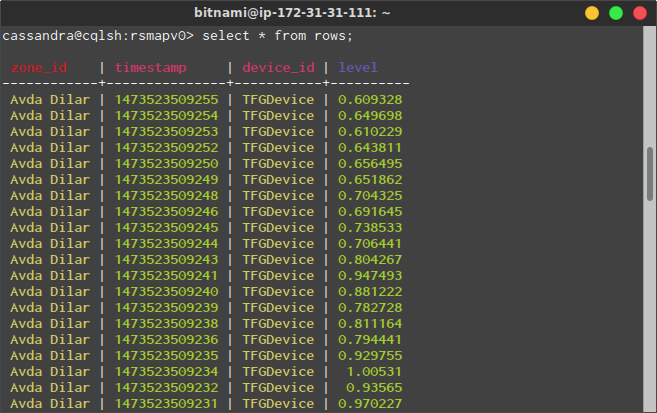
\includegraphics[scale=0.65]{../images/cassandra/6.png}
		\caption{Cassandra con datos almacenados}
    \label{fig:kaa}
	\end{center}
\end{figure}

Para finalizar vamos a crear dos funciones en java dentro del Keyspace que nos ayudarán a visualizar y consultar los datos posteriormente. La necesidad de definir estas funciones viene dada porque el campo TimeStamp se almacena bajo el formato UnixTimestamp que nosproporciona los milisegundos actuales transcurridos desde 1970. Es importante destacar que estas funciones pueden ser definidas en el lenguaje que queramos, en nuestro caso vamos a usar Java.

\bigskip

La primera convierte un \textit{timestamp} en una hora legible, las otras dos nos ayudarán a seleccionar los datos de un minuto atrás hasta la fecha actual y de una hora atrás hasta la fecha actual.

\begin{figure}[!ht]
  \begin{center}
    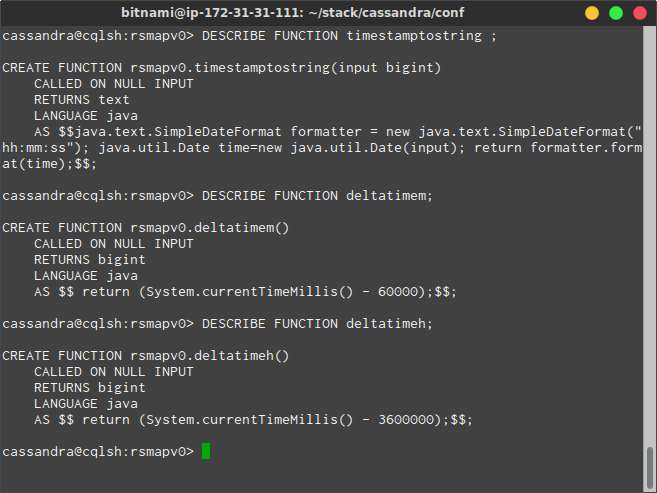
\includegraphics[scale=0.65]{../images/cassandra/5.png}
		\caption{Funciones dentro de Cassandra}
    \label{fig:kaa}
	\end{center}
\end{figure}

\newpage

Si queremos hacer uso de éstas funciones debemos editar el fichero \textbf{/home/bitnami/stack/cassandra/conf} y cambiar la línea:

enable user defined functions: false

por:

enable user defined functions: true

\bigskip

Ya sólo nos queda reiniciar el servicio:

\begin{lstlisting}[language=bash,caption={Reiniciando Cassandra},label={lst:rcas}]
	$ sudo ./stack/ctlscript.sh stop cassandra
	$ sudo ./stack/ctlscript.sh start cassandra
\end{lstlisting}

A modo de resumen, hasta el momento tenemos la plataforma KAA desplegada, en ella se encuentra el esquema de datos a usar y el LogAppender que indica a donde se van a remitir los datos. Además tenemos Apache Cassandra desplegado y con las tablas necesarias creadas para empezar a enviar información de las señales detectadas. Ésto quiere decir estamos en disposición de generar el SDK que usarán los clientes para connectarse a Cassandra.

\bigskip

Para generar el SDK accedemos a la interfaz web de KAA. Los SDK's se generan bajo un sistema de versiones lo que nos posibilita tener varios para una misma aplicación con distinto funcionamiento. El control de éstas versiones se gestiona mediante perfiles SDK por lo que si queremos obtener el nuestro debemos definir en primer lugar un perfil en el que también se deben especificar las versiones para los esquemas y log appenders.

Una vez nos encontremos en la interfaz buscamos la aplicación creada que se detalló en la sección de \textit{Configuración de KAA} y nos situamos en la opción \textit{SDK profiles} / \textit{Add SDK Profile}.


\begin{figure}[!ht]
  \begin{center}
    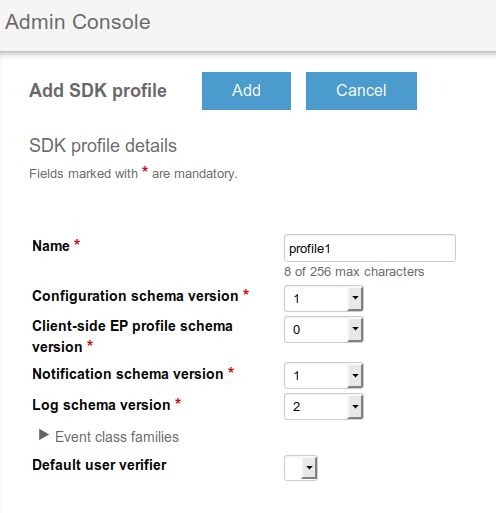
\includegraphics[scale=0.30]{../images/sdk/1.png}
		\caption{Definición del SDK}
    \label{fig:kaa}
	\end{center}
\end{figure}

\newpage

Por último pulsamos la opción \textit{Generate SDK} la cual nos muestra una ventana en la que debemos escoger sobre qué lenguaje se generará el SDK. RSMap usa el SDK generado en Java.


\begin{figure}[!ht]
  \begin{center}
    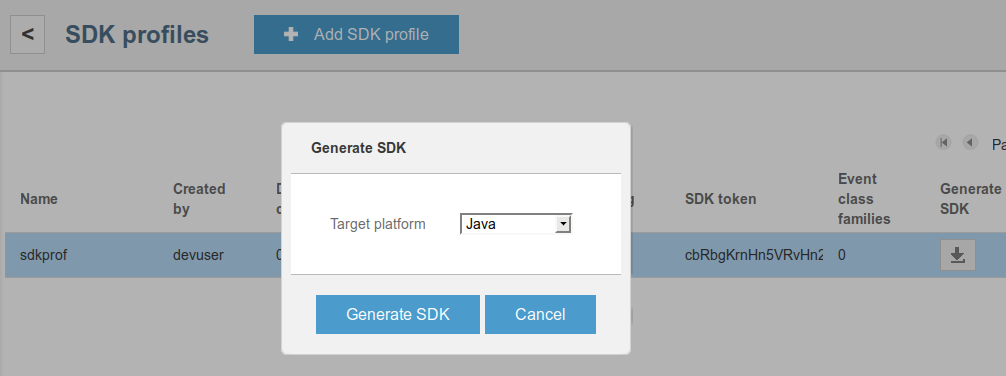
\includegraphics[scale=0.30]{../images/sdk/2.png}
		\caption{Definición del SDK}
    \label{fig:kaa}
	\end{center}
\end{figure}

\newpage

\section{Desarrollo del módulo de detección de vehículos.}

El código completo de éste módulo se encuentra en el repositorio \url{https://github.com/RSMap/RSMapPi}, dentro de la organización \url{https://github.com/RSMap} que alberga el proyecto RSMap completo.

\bigskip

Para analizar la estructura podemos hacer una clara división en dos partes, por un lado tenemos el módulo en python que se encarga de interactuar con la tarjeta de sonido, tomar los datos y enviarlos. La segunda parte es el módulo en java que se encarga de usar el SDK generado en KAA para enviarlos a Cassandra.

\subsection{Módulo de detección}

Para detallarlo de una manera clara se analizarán fragmentos de código separadamente, aunque todos ellos pertenecen al mismo archivo \textit{(RSMapPi/\/analyzer/\/VehicleDetection.py)} pero antes a modo de resumen se enumeran las librerías más reseñables y la secuencia que sigue el programa a lo largo de su ejecución.

\subsubsection{Dependencias}

Las dependencias externas y necesarias de éste módulo se encuentran especificadas en el archivo \textit{(RSMapPi/\/analyzer/\/requirements.txt)}. Las más importantes son:

\begin{itemize}
	\item \textbf{sounddevice==0.3.4:} es la más importante ya que mediante ella se accede al dispositivo para capturar los datos. Hay que destacar que los ejemplos de su documentación han sido de gran ayuda a la hora del desarrollo de éste módulo.
	\item \textbf{numpy==1.11.1:} es la librería por excelencia para el análisis científico de datos en Python.
	\item \textbf{requests==2.11.1:} nos proporciona una cómoda interfaz para efectuar peticiones HTTP que serán usadas para interactuar con la API Rest.
\end{itemize}

\newpage

Además se han usado algunas otras dependencias pertenecientes a python, su instalación no es necesaria pues vienen con el compilador del lenguaje, ellas son:

\begin{itemize}
	\item \textbf{queue:} contine la estuctura de datos de cola, sobre la que se insertaran y leerán los datos obtenidos.
	\item \textbf{threading:} nos permite crear hebras y procesos.
	\item \textbf{socket:} nos servirá para enviar los datos obtenidos desde Python al SDK de KAA que, recordemos que está en Java.
\end{itemize}

\bigskip

\subsubsection{Resumen de ejecución}

\bigskip

En primer lugar se realiza una petición a la API para dar de alta el dispositivo en la lista de los receptores que se encuentran enviando datos. Si esa petición nos devuelve el código 400 significa que ese dispositivo ya se encuentra dado de alta, por lo que en ese caso vamos a realizar otra petición, ésta vez sobre la ruta asignada a ese dispositivo en concreto para indicar que el dispositivo se ha conectado y empezará a retransmitir datos en breve. En caso de que el dispositivo no exista, se da de alta con el payload que contiene toda la información asociada a el.

\bigskip

Una vez el dispositivo se identifica mediante la API, se abre un socket sobre el mismo equipo (localhost), éste servirá para enviar los datos obtenidos desde Python a Java. Los dos primeros mensajes que se envían son la cadena de localización del dispositivo y su identificador.

\bigskip

A continuación se definen una serie de variables que serán usadas para la detección y análisis del tráfico.
Tras ésto se lanzan dos hebras, una trabajará con la función \textit{producer} y la otra con la función \textit{consumer}.

\bigksip

La hebra \textit{producer} hace uso de la librería \textbf{Sound device} a la que llama con los parámetros definidos anteriormente, el más destacable es callback, que hace referencia a la función \textit{callback} la cual tiene el cometido generar los bloques con los datos numéricos extraidos desde la tarjeta de sonido y ponerlos en la cola.
\bigskip

La hebra \textit{consumer} es la encargada de analizar la información puesta en la cola y enviar las señales tanto al SDK (valores que se almacenarán) como a la API Rest (valores que se representarán en el mapa). Cuando el programa recibe una señal de interrupción (\textit{enter, 'q' o 'Q'}) el productor pondrá en la cola un objeto de llamado \textit{\_sentinel} el cual le indicará al consumidor que el programa va a finalizar. El consumidor envía las señales de parada a la API Rest, que borrará el dispositivo de la lista de dispositivos retransmitiendo así como al programa en Java que cerrará la conexión con Cassandra.

\newpage
\subsubsection{Código}

Al comienzo del fichero se definen una serie de variables que serán usadas cuando el dispositivo envíe información. Gracias a ellas éste quedará identificado por un id (\textit{device\_id}), una localización en formato texto (\textit{device\_location}) y una localización geográfica (\textit{latitude y longitude}).

A continuación se generan los payloads iniciales que se usarán para realizar las peticiones sobre la API, éstos tiene estructura de map \{'clave' : valor\} y tenemos dos tipos:

\begin{itemize}
	\item \textbf{new\_device\_payload:}

	contiene toda la información asociada al dispositivo, es usado cuando el dispositivo no está registrado en la plataforma web.
	\item \textbf{existing\_device\_payload:}

	contiene únicamente el nivel iniciado a -1, ésto permitira identificarlo como nuevo dispositivo y representarlo en el mapa con un icono que indique una nueva conexión.
\end{itemize}

En la parte final de éste bloque se definen las URLS que se necesitarán para comprobar el estado del dispositivo en el sistema.

\begin{itemize}
	\item \textbf{signals\_list\_url: }

	referencia a la url que contiene todos los dispositivos registrados.
	\item \textbf{signal\_url: }

	referencia a la url que identifica un dispositivo en concreto.
\end{itemize}

\begin{lstlisting}[language=python,caption={Parámetros usados para la comunicación con la API},label={lst:pi1}]
	# device id (case sensitive)
	device_id = 'TFGDevice'
	# device location (name)
	device_location = 'Avda Dilar'
	# device coordinates
	latitude = '37.177336'
	longitude = '-3.598557'
	# signal_type (default unknown)
	signal_type = 'u'
	# level -1 means device is connected and it will send data soon.
	level = '-1.0'
	# new_device_payload contains all related info with a map structure
	new_device_payload = {'device_id':device_id, 'lat':latitude, 'long':longitude, 'level':level, 'type':signal_type}
	# if device exists, only level is needed
	existing_device_payload = {'level': level}
	# rest urls
	signals_list_url = 'http://52.210.3.41/api/signals/'
	signal_url = 'http://52.210.3.41/api/signal/'+device_id+'/'
\end{lstlisting}

El siguiente bloque se encarga de hacer uso de las URL's y Payloads definidos anteriormente

\begin{lstlisting}[language=python,caption={Identificación de dispositivo mediante la API},label={lst:pi1}]
# rest first request
req = requests.post(signals_list_url, new_device_payload)

# check rest response
if(req.status_code == 400):
    print("Device already exists, sending connect signal")
    req = requests.patch(signal_url, existing_device_payload)
    if(req.status_code == 200):
        print("Connection successful")
    else:
        print("Can't send connected signal, exiting")
        sys.exit()
elif(req.status_code == 201):
    print("Connection successful, device added to device's database")
else:
    print("Device can't connect to rest service, check your connection.")
    sys.exit()
\end{lstlisting}

Cuando realizamos una petición HTTP obtenemos un valor numérico que nos indica el resultado de dicha petición. En base a los códigos obtenidos podemos saber si el dispositivo se encontraba dado de alta, por lo que no se puede sobreescribir con una petición POST (\textit{código 400}) o por el contrario si se añadió satisfactoriamente (\textit{código 201}).

En el caso de no poder realizar la petición POST usamos la petición PATCH que básicamente es un \textit{update} sobre el objeto en Django que contiene la información del dispositivo, es aquí donde se usa la URL definida en la variable \textit{signal\_url} que hace referencia directa al dispositivo en cuestión.

En cualquier caso, el campo \textit{level} será establecido a -1, lo que sobre el mapa se traducirá en el icono de conexión.

\newpage

El siguiente paso es conectarse al Socket creado por \textit{DataSender.java} que deberá estar lanzado y esperando conexiones.

\begin{lstlisting}[language=python,caption={Conexión con Java mediante un Socket},label={lst:pi1}]
	# Connecting to DataSender socket on localhost
	socket = socket.socket()
	socket.connect(('localhost', 5000))
	# Send device location
	device_location_sock = device_location+"\n"
	device_location_bytes = bytes(device_location_sock, 'utf-8')
	socket.send(device_location_bytes)
	# Send device id
	device_id_sock = device_id+"\n"
	device_id_bytes = bytes(device_id_sock, 'utf-8')
	socket.send(device_id_bytes)
\end{lstlisting}

Se le envían dos mensajes iniciales que contienen la cadena de localización y el id del dispositivo los cuales serán usados a posteriori por \textit{DataSender.java} para añadirlos a Cassandra. No se puede pasar una cadena como tal, es por eso por lo que se convierten en Bytes antes de enviarlos.

\bigskip

Ahora se definen las variables necesarias para la captura e identificación de vehículos.

\begin{lstlisting}[language=python,caption={Variables corresopndientes al análisis},label={lst:pi1}]
 # multiplier factor
 gain = 10
  # number of cuantization levels
 levels = 100
 # system device id
 device = 2
 # block time (ms)
 block_duration = 100
 # sample rate
 samplerate = 44100
 # high sample rate
 high = 2000
 # low sample rate
 low = 450
 # cuantization value
 delta_f = (high - low) / levels
 # window will divided in bands, fftsize defines the resolution on freq domain
 fftsize = np.ceil(samplerate / delta_f).astype(int)
 # window freq resolution
 low_bin = np.floor(low / delta_f)
 # vehicle threshold
 threshold = 0.59
 # consequtive blocks, its may depend of the road conditions
 consequtive_blocks = 50
\end{lstlisting}

Las variables \texit{threshold} y \texit{consequtive\_blocks} tienen relación directa con la identificación de vehículos. La primera indica el umbral mínimo que deben tener los valores obtenidos por cada bloque obtenido mientras que la segunda indica qué número de bloques necesitamos por encima de ese umbral para considerar que un vehículo ha pasado.

El resto poseen la misma estructura que las del ejemplo que proporciona la librería \textit{SoundDevice} para cuantizar los valores obtenidos através de una entrada de audio. ( \url{http://python-sounddevice.readthedocs.io/en/0.3.4/examples.html#real-time-text-mode-spectrogram} )


\bigskip

La esencia de la hebra productora es la llamada a \textbf{InputStream} que abre un canal de comunicación con la tarjeta de sonido. Toma como argumentos los valores definidos anteriormente y una función llamada \textit{callback}, que es la encargada de generar cada bloque y ponerlo en la cola. Cada bloque consta de una serie de valores que tras aplicarle la Transformada Rápida de Fourier son sumados obtenieno así el valor global para cada bloque.

\begin{lstlisting}[language=python,caption={Hebra productora},label={lst:pi1}]
with sd.InputStream(
	device=device,
	channels=1,
	callback=callback,
	blocksize=int(samplerate * block_duration / 1000),
	samplerate=samplerate
)
\end{lstlisting}

\bigskip

El código perteneciente a la hebra consumidora consiste en un bloque que se ejecuta mientras no obtenga una señal de parada, en tal caso se envía una señal de desconexión a la API usando el método DELETE que eliminará el modelo asociado al dispositivo en Django y otra a \textit{DataSender.java}. El código encargado de filtrar los datos es el siguiente:

\begin{lstlisting}[language=python,caption={Hebra consumidora},label={lst:pi1}]
if(data > threshold ):
	# global block consequtive count
	consequtive += 1
	local_consequtive += 1
	local_data_sum += data
	if(local_consequtive == consequtive_blocks):
		# if detected > consequtive_blocks send to api rest
		existing_device_payload = {
			'level': str(local_data_sum)
		}
		req = requests.patch(signal_url, existing_device_payload)

		print(
			str(consequtive_blocks) +
			" consequtive blocks, sending to rest API "
			+ str(local_data_sum)
			)
		local_consequtive = 0
		local_data_sum = 0.0

		# add representative values to send_queue
		send_queue.put(data)
else:
	if(consequtive > consequtive_blocks):
		print("Sending data to cassandra")
		while not send_queue.empty():
			# detected case, sending items to KAA SDK via TCP socket
			item_to_send = send_queue.get()
			linestr =str(item_to_send)+"\n"
			linebytes = bytes(linestr, 'utf-8')
			socket.send(linebytes)

	# consequtive was not bigger than consequtive_blocks, cleaning resources
	send_queue = Queue()
	send_queue.queue.clear()
	consequtive = 0
	local_consequtive = 0
	local_data_sum = 0.0
\end{lstlisting}

Si el dato obtenido de la cola supera el umbral definido incrementaremos la variable que indica los bloques consecutivos válidos hasta el momento, además añadiremos el valor a una suma parcial. En cuanto tengamos un número de bloques válido efectuaremos una petición PATCH a la API que actualizará el valor para el dispositivo con la suma total de los bloques obtenidos. Por último éste valor se situa en otra cola que alimentará a la aplicación \textit{DataSender.java}.

El motivo de enviar ésta señal cuando detectamos los bloques necesarios es para garantizar que la aplicación trabaja en tiempo real sobre el mapa, los datos que se envían a \textit{DataSender.java} pueden sufrir pequeños retrasos debio a que éstos se envían cuando se obtiene un valor que no supera el umbral. Tras enviarlos todos los recursos que ocupan son liberados para proceder a la detección de un nuevo vehículo.

\newpage

Las funciones \textit{producer} y \textit{consumer} son llamadas cuando se inicializan los Threads correspondientes a cada una de ellas.

\begin{lstlisting}[language=python,caption={Inicialización de las hebras},label={lst:pi1}]
	queue = Queue()

	# thread instances
	thread_prod = Thread(target=producer, args=(queue, ))
	thread_cons = Thread(target=consumer, args=(queue, ))

	# thread init
	thread_prod.start()
	thread_cons.start()

\end{lstlisting}

\newpage

\subsection{Módulo de envío}

Éste módulo se encargará de de inicializar el Socket necesario para que \textit{VehicleAnalyzer.py} le proporcione los datos que posteriormente enviará a Cassandra. La estructura es más simple que la del módulo anterior en gran medida a que el SDK que proporciona KAA tiene una interfaz muy cómoda para trabajar con ella.

\subsubsection{Dependencias}

Las dependencias necesarias son el SDK generado por KAA en formato \textit{.JAR} así como otras dependencias ajenas pertenecientes a KAA. Todas ellas se encuentran bajo el directorio \textit{sender} y se pueden identificar con los siguientes nombres:

\begin{itemize}
	\item kaa-java-ep-sdk.jar
	\item log4j-over-slf4j-1.7.7
	\item logback-classic-1.1.2
	\item logback-core-1.1.2
\end{itemize}

\subsubsection{Resumen de ejecución}

La primera tarea inicia el cliente KAA \texit{kaaClient} sobre el cual se enviarán los datos.

Lo siguiente es inicializar el Socket y esperar la llegada de mensajes, los dos primeros indicarán localización e id como se indicó anteriormente.

Mientras no se detecte una señal de parada (\textit{carácter 'q'}) el Socket estará aceptando conexiones y leyendo los datos de cada una.

Para cada conexion crea un objeto de la clase \textit{AudioReport}, éste nombre y sus atributos vienen definidos por los esquemas que definimos anteriormente sobre la plataforma KAA. Tras asociarle los valores pertinentes el objeto es enviado gracias a la función \textit{addLogRecord(report);} que añadirá éste objeto en forma de entrada a Cassandra.

\newpage

\subsubsection{Código}

En el siguiente fragmento de código se detalla como se abre el Socket y se leen las dos primeras entradas asociandolas a las variables pertinentes

\begin{lstlisting}[language=python,caption={Inicialización del Socket},label={lst:pi1}]
	ServerSocket Server = new ServerSocket (5000);

	System.out.println ("Waint for VehicleAnalyzer on TCP socket at port 5000");

	// Listening connections
	Socket connected = Server.accept();
	System.out.println( " VehicleAnalyzer with "+ connected.getInetAddress() +":"+connected.getPort()+" is connected! ");

	// Init reading buffer over TCP socket
	BufferedReader inFromClient = new BufferedReader(new InputStreamReader (connected.getInputStream()));

	// First two packets comes with device location and device id
	String location = inFromClient.readLine();
	String device = inFromClient.readLine();
\end{lstlisting}

Para finalizar se muestra la creación y envío del objeto que se traducirá en una fila dentro de nuestra base de datos.

\begin{lstlisting}[language=java,caption={Creación y envío de datos a Cassandra},label={lst:pi1}]
	// create new AudioReport object wich is appended to Cassandra
	AudioReport report = new AudioReport();
	long timestamp = System.currentTimeMillis();
	report.setZoneId(location);
	report.setDeviceId(device);
	report.setLevel(Double.parseDouble(fromclient));
	report.setTimestamp(timestamp);

	// send Audio Report object
	kaaClient.addLogRecord(report);
\end{lstlisting}

\newpage


\section{Desarrollo de la plataforma web.}

La estructura de la plataforma web se detalló en el capítulo de diseño, por tanto vamos a proceder a analizar los archivos más relevantes que la componen. Al igual que el módulo de detección podemos hacer una distinción clara entre las dos partes que la componen, la web de RSMap y la API Rest.

\subsection{Plataforma web}

\subsubsection{Dependencias}

Se encuentran especificadas en el archivo \textit{(RSMap\/requirements.txt)} dentro del repositorio \url	{https://github.com/RSMap/RSMap}

\begin{itemize}
	\item \textbf{Django==1.10.1}
\end{itemize}

\subsubsection{Código}

Los archivos de Django que disponen el comportamiento de la aplicación (parte lógica) son \textbf{models.py} en el que se define la estructura de datos que será almacenada, tiene un formato como el que se muestra a continuación:


\begin{lstlisting}[language=python,caption={Modelo definidos en Django},label={lst:pi1}]
class Signal(models.Model):
  device_id = models.TextField(primary_key=True)
  lat = models.DecimalField(max_digits=9, decimal_places=6)
  long = models.DecimalField(max_digits=9, decimal_places=6)
  created = models.DateTimeField(auto_now=True, blank=True)
  level = models.FloatField()

  type = models.CharField(
      max_length = 1,
      choices = VEHICLE_TYPE,
      default = UNKNOWN,
  )

  def __str__(self):
  	return self.device_id
\end{lstlisting}

Un campo a tener en consideración es el llamado \textit{created}, en concreto el argumento \textbf{auto\_now=True} que nos va a permitir que cada vez que un objeto almacenado del tipo \textit{Signal} sea creado o actualizado, el valor de éste campo será actualizado con el \textit{timestamp} relativo a la fecha de dicho cambio. Así podremos tener constancia de cual fué el último momento en el se actualizo, por ejemplo, el campo \textit{level}.


\newpage
El siguiente fragmento de código pertenece al archivo \textit{urls.py} en el que se definirán las rutas que va a proporcionar RSMap en su web:

\begin{lstlisting}[language=java,caption={Definición de URL's},label={lst:pi1}]
urlpatterns = format_suffix_patterns([
  url(r'^api/signals/$', views.SignalList.as_view(), name='signal-list'),
  url(r'^api/signal/(?P<pk>[a-zA-Z0-9]+)/$', views.SignalDetail.as_view(), name='signal-detail'),
  url(r'^$', TemplateView.as_view(template_name='index.html')),
  url(r'^map/$', TemplateView.as_view(template_name='map.html')),
])
\end{lstlisting}

Éstas URL's se definen mediante expresiones regulares, si en el navegador se introduce una URL que entra del patrón de una de éstas expresiones, se llamará a la vista correspondiente para esa URL.

Tanto las URL's pertenecientes a la web, como las pertenecientes a la API Rest son definidas en éste mismo fichero.

\bigskip

Los directorios \textit{static} y \textit{templates} son los encargados de crear la parte visual de la web de RSMap.

En \textit{templates} podemos encontrar las plantillas que sirve nuestra aplicación, ambas usan HTML5 y Bootstrap:

\begin{itemize}
	\item \textbf{index.html:} contiene la página principal.
	\item \textbf{map.html:} contiene la página con el mapa de tráfico.
\end{itemize}

\bigskip

Dentro del fichero \textit{map.html} se incluye el archivo \textit{static\//js\//rsmapMapUpdater.js} que se encargará de actualizar dinamicamente el contenido del mapa.

La funcion \textit{checkDevices} se ejecuta cada 30 segundos y permite a un visitante saber si existen dispositivos retransmiendo en ese momento, en caso de que no se le mostrará una indicación de ello en la esquina superior derecha.

\newpage

\begin{lstlisting}[language=javascript,caption={Función checkDevices},label={lst:pi1}]
function checkDevices(){
  $(function(){
      $.getJSON('http://52.210.3.41/api/signals.json', function(data) {
          if(data.length == 0){
            bootstrap_alert.warning('<strong>INFO:</strong> No devices sending data right now', 'warning', 4000);
          }
      });
  });
}
\end{lstlisting}

En el siguiente fragmento se muestra como se actualiza el mapa. El proceso consta de dos pasos.

Cada segundo se comprueba la ruta \textit{http://52.210.3.41/api/signals.json} que devuelve la lista de dispositivos conectados a RSMap. Una vez se ha obtenido se recorre esa lista y se comprueban los tiempos en los que fueron añadidos, si éstos tiempos pertenecen al intervalo \textit{(tiempo actual - 2 segundos) > timestampSeñal > (tiempo actual)} se procede a representarla en el mapa.

\begin{lstlisting}[language=javascript,caption={Actualización dinámica del mapa},label={lst:pi1}]
// map update via AJAX
$(document).ready(
  function worker(){
	  $.ajax(
	    {
	      // retrieve updated json with last valid signals
	      url:"http://52.210.3.41/api/signals.json",

	      complete: function(){
	        // next call will be in 1 second
	        setTimeout(worker, 1000);
	      }
	    }
    ).then(
      function(data)
      {
        //clean map
        deleteMarkers();

        // run all json markers and add them to map
        for(var i = 0; i < data.length; i++){
          var signal = data[i];
          //console.log(signal);

          var signal_timestamp = parseFloat(signal['created']);
          // convert now to seconds and 2 seconds less
          // (python timestamp comes in seconds)
          // that's the reason to divide by 1k
          var now = ((new Date().getTime()-2000)/1000|0) ;

          // update 'last update' field
          $('.last-update').empty();
          var now_date = new Date();
          $('.last-update').append(now_date);

          // now was reduced 2 seconds so if signal_timestamp is greather than
          // now means it was in a interval between now and 2 secs later
          if(signal_timestamp > now){
            var location = new google.maps.LatLng(parseFloat(signal['lat']), parseFloat(signal['long']));
            var level = signal['level'];
            addMarker(location, level);
          }
        }
      }
    );
  }
);
\end{lstlisting}

Para cada señal que se va a representar se tiene su valor \textit{level}. Según el tamaño de éste valor se representará la señal en el mapa con distintos iconos.

\begin{figure}[!ht]
  \begin{center}
    
\includegraphics[scale=1]{../images/map/0.png}
		\caption{Icono para valor -1: conexión de dispositivo}
    \label{fig:kaa}
	\end{center}
\end{figure}

\begin{figure}[!ht]
  \begin{center}
    
\includegraphics[scale=1]{../images/map/1.png}
		\caption{Icono para valor \textgreater 55.5: vehículo pesado}
    \label{fig:kaa}
	\end{center}
\end{figure}

\begin{figure}[!ht]
  \begin{center}
    
\includegraphics[scale=1]{../images/map/2.png}
		\caption{Icono para valor 45.5 \textless x \textless 55.5: vehículo medio}
    \label{fig:kaa}
	\end{center}
\end{figure}

\begin{figure}[!ht]
  \begin{center}
    
\includegraphics[scale=1]{../images/map/3.png}
		\caption{Icono para valor x \textless 45.5: vehículo ligero}
    \label{fig:kaa}
	\end{center}
\end{figure}

En un principio se pensó en efectuar ésta comprobación en la parte lógica de la aplicación pero como los datos se obtienen de todas formas en el cliente, se aprovecha ésta situación para realizar la comprobación en el navegador de éste modo se libera carga del servidor web.

\subsection{API Rest}

\subsubsection{Dependencias}

Dentro del mismo repositorio, en el mismo archivo \textit{requirements.txt} se encuentra la linea necesaria para la API.

\begin{itemize}
	\item \textbf{djangorestframework==3.4.6}
\end{itemize}

\subsubsection{Código}

Tanto el archivo \textit{models.py} como el \textit{urls.py} son usados por la API, que forma parte del ecosistema que genera Django, por tanto vamos a definir los archivos que componen la API.

\bigskip

El primer archivo se llama \textit{serializers.py} y en el se detalla cómo se va a usar el modelo \textit{Signal} en la API, es decir, cuando una petición solicite un objeto de tipo \textit{Signal} qué campos se devolveran en el JSON.

\begin{lstlisting}[language=python,caption={Serializador del modelo Signal},label={lst:pi1}]
class SignalSerializer(serializers.ModelSerializer):
  created = serializers.DateTimeField(format="%s", required=False)

  class Meta:
    model = Signal
    fields = ('device_id','lat','long','created','level','type',)
\end{lstlisting}

\bigskip

Para finalizar el archivo \textit{views.py} definimos las vistas que tendrá nuestra API, dos como se ha mencionado anteriormente. La primera de ellas devuelve un JSON con todos los dispositivos conectados a RSMap y la segunda los campos para un dispositivo en concreto.

Éstas vistas son llamadas desde las urls que servirán la API y que fueron descritas anteriormente cuando se expuso el archivo \textit{urls.py}.

\begin{lstlisting}[language=python,caption={Vistas de la API},label={lst:pi1}]
class SignalList(generics.ListCreateAPIView):
  queryset = Signal.objects.all()
  serializer_class = SignalSerializer

class SignalDetail(generics.RetrieveUpdateDestroyAPIView):
  queryset = Signal.objects.all()
  serializer_class = SignalSerializer
\end{lstlisting}

\newpage


\section{Instalación y configuración de Apache Zeppelin.}

\subsection{Instalación}
Es hora de instalar Apache-Zeppelin. Como en los servicios anteriores, lo primero que debemos hacer es configurar e iniciar una nueva instancia en Amazon EC2. Los pasos a seguir son los mismos con la salvedad de la selección de la imagen y la configuración de \textit{Security groups}.

\bigskip

El SO usado ésta vez será Ubuntu 14.04.4 LTS, para seleccionarlo lo podemos buscar dentro de las imágenes disponibles al configurar la nueva instancia.

Como tráfico entrante abriremos el puerto 8080 que es donde se va a ejecutar Apache-Zeppelin.

Una vez que tengamos la máquina disponible accedemos por SSH y procedemos a instalar Apache-Zeppelin con las siguientes órdenes:

\begin{lstlisting}[language=bash,caption={Instalación de Apache-Zeppelin},label={lst:pi1}]
$ cd /opt
$ sudo wget http://apache.rediris.es/zeppelin/zeppelin-0.6.1/zeppelin-0.6.1.tgz
$ sudo tar -zxvf zeppelin-0.6.1.tgz
$ sudo /opt/zeppelin-0.6.1-bin-all/zeppelin-daemon.sh
\end{lstlisting}

Debemos asegurarnos de descargar el binario que trae los intérpretes instalados, entre ellos el de Cassandra para poder hacer llamadas a la base de datos en los Notebooks.

Si ahora abrimos el navegador a nuestra dirección pública deberíamos encontrarnos con lo siguiente:

\begin{figure}[!ht]
  \begin{center}
    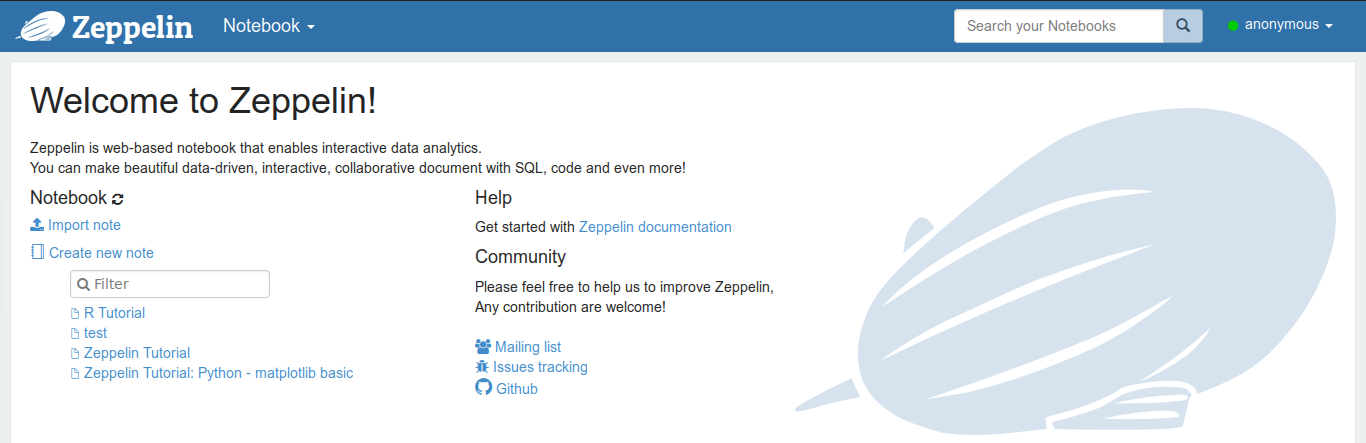
\includegraphics[scale=0.30]{../images/zeppelin/1.png}
		\caption{Apache Zeppelin en funcionamiento}
    \label{fig:kaa}
	\end{center}
\end{figure}

\subsection{Configuración}

Vamos a configurar es el intérprete de Cassandra, para ello nos dirigimos a la parte derecha de la interfaz y entramos en la opción \textit{interpreters}. Tras localizar el intérprete de Cassandra pulsamos el botón \textit{editar} y configuramos los siguientes campos:

\begin{itemize}
\item \textbf{cassandra.credentials.password, } aquí indicamos la contraseña de Cassandra.
\item \textbf{cassandra.credentials.username, } aquí el usuario.
\item \textbf{cassandra.hosts, } aquí la dirección pública del servidor de Cassandra.
\item \textbf{cassandra.keyspace , } y aquí el Keyspace que definimos anteriormente en Cassandra.
\end{itemize}

para finalizar guardamos los cambios efectuados.

Ahora estamos preparados para crear un nuevo Notebook para RSMap mediante el menú desplegable \textit{Notebooks} y la opción \textit{create new notebook} al cual deberemos establecer un nombre. Una vez hecho ésto entraremos en el Notebook que tiene una estructura como muestra la \textit{figura 6.20}.

\begin{figure}[!ht]
  \begin{center}
    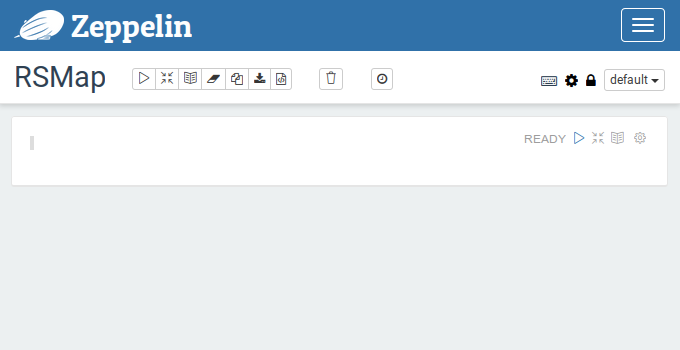
\includegraphics[scale=0.50]{../images/zeppelin/2.png}
		\caption{Estructura de un Notebook en Zeppelin}
    \label{fig:kaa}
	\end{center}
\end{figure}

Sólo queda una tarea por realizar, que es configurar cuales de los intérpretes estarán disponibles para usar bajo este Notebook.
Existen muchos como el de \textit{Scala, Python, Java o Markdown} entre otros.

Para configurarlos nos dirigimos a la rueda dentada situada en la parte derecha y desactivamos todos los intérpretes a excepción de el de Cassandra. La configuración debe quedar tal que así:

\begin{figure}[!ht]
  \begin{center}
    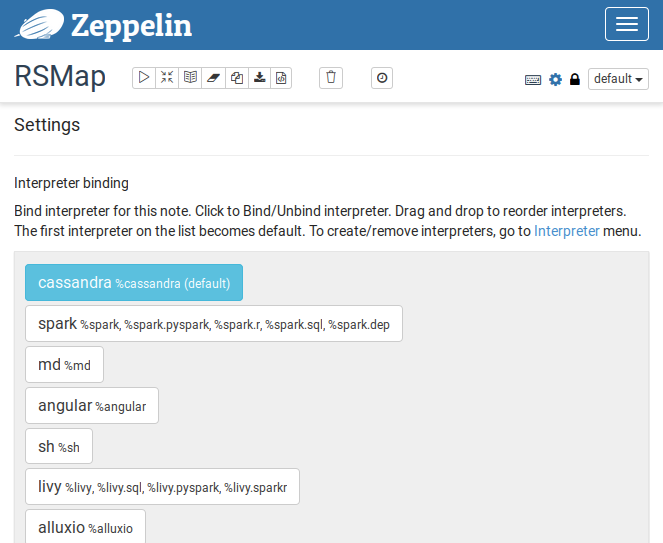
\includegraphics[scale=0.50]{../images/zeppelin/3.png}
		\caption{Cassandra como intérprete para Zeppelin}
    \label{fig:kaa}
	\end{center}
\end{figure}

\newpage

Ya tenemos todos los elementos preparados para realizar consultas en \textit{CQL} a nuestro servidor Cassandra y poder visualizar los datos. La interfaz de Zeppelin está compuesta de varias celdas en las cuales podemos introducir el código deseado.

En nuestro caso estas sentencias pertenecen al intérprete de Cassandra luego la primera línea de cada celda debe contener la palabra clave \textbf{\%cassandra}. Una vez tengamos escrita la consulta podemos pulsar el botón de \textit{Play} y esperar unos segundos para obtener los resultados.

\bigskip

Vale la pena destacar que Zeppelin posee un sistema de programación de tareas al que podemos acceder pulsando el pequeño icono del reloj llamado \textit{Run scheduler} con una estructura similar a crontab, ésto nos permite programar un tiempo predeterminado para que se ejecuten las celdas del Notebook de manera automática y poder tener los resultados actualizados en todo momento.

\subsection{Ejemplo de consulta CQL}

Detallamos un ejemplo de consulta a modo de ilustración de como funciona CQL, veamos que forma tiene y posteriormente se comentarán las diferentes partes de la misma.

\begin{lstlisting}[language=cql,caption={Ejemplo de consulta CQL},label={lst:json_personal}]
%cassandra
SELECT rsmapv0.timestampToString(timestamp) AS time, level from rsmapv0.rows WHERE zone_id={{zone_id='Granada'}} and timestamp > rsmapv0.deltatimeH() ORDER BY timestamp ASC;
\end{lstlisting}

Como se vió en la parte de configuración de Cassandra habíamos creado ciertas funciones para usarlas a la hora de consultar los datos, es el momento de verlas en funcionamiento. \textit{rsmapv0.timestampToString} es la función que nos formatea un \textit{timestamp} a una fecha, rsmapv0 indica en que Keyspace se encuentra dicha función.

En la cláusula WHERE tenemos \textbf{ zone id = \{\{zone id='Granada'\}\}} lo que nos permitirá modificar el valor de ese campo mediante la interfaz de Zeppelin si necesidad de reescribir la consulta.

En último lugar \textbf{rsmapv0.deltatimeH()} hace referencia a una de las otras funciones definidas en Cassandra, en este caso se indica en la consulta que el campo \textit{timestamp} debe ser mayor que \textbf{rsmapv0.deltaTimeH}. Ésta función nos devuelve la hora actual restándole un minuto, por tanto obtendremos todos los valores de un minuto antes de la fecha actual.

\bigskip

Tras poner el sistema en funcionamiento durante un minuto en el que pasan algunos vehículos podemos ver como Zeppelin representa los datos mediante la consulta mencionada:

\begin{figure}[!ht]
  \begin{center}
    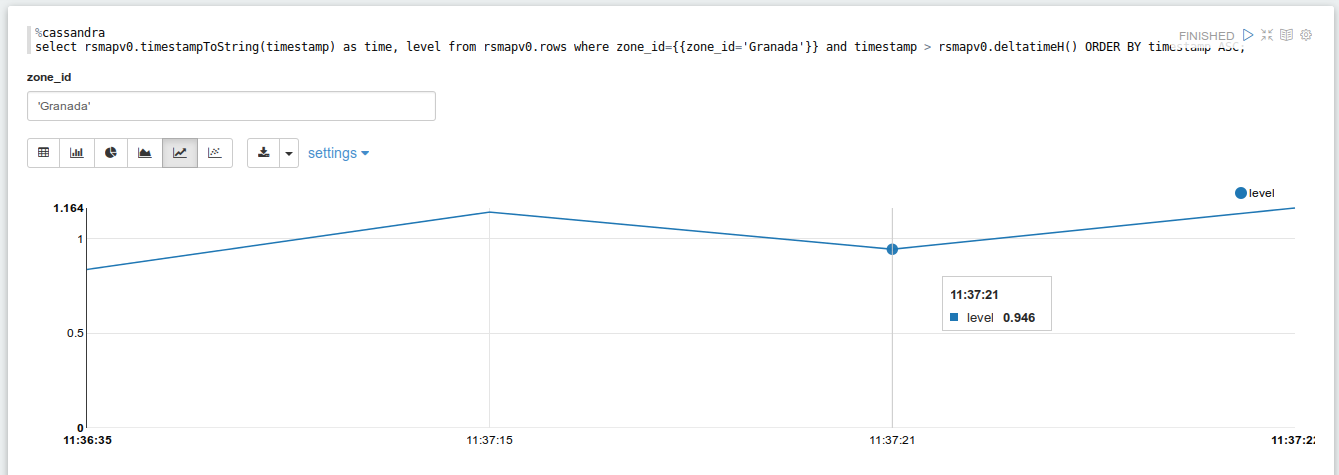
\includegraphics[scale=0.30]{../images/zeppelin/4.png}
		\caption{Muestra de resultados en Zeppelin}
    \label{fig:kaa}
	\end{center}
\end{figure}

\newpage
